% Created 2021-09-23 Thu 17:27
% Intended LaTeX compiler: pdflatex
\documentclass[presentation]{beamer}
\usepackage[utf8]{inputenc}
\usepackage[T1]{fontenc}
\usepackage{graphicx}
\usepackage{grffile}
\usepackage{longtable}
\usepackage{wrapfig}
\usepackage{rotating}
\usepackage[normalem]{ulem}
\usepackage{amsmath}
\usepackage{textcomp}
\usepackage{amssymb}
\usepackage{capt-of}
\usepackage{hyperref}
\usepackage[UTF8]{ctex}
% TIPS
% \substack{a\\b} for multiple lines text





% pdfplots will load xolor automatically without option
\usepackage[dvipsnames]{xcolor}

\usepackage{forest}
% two-line text in node by [two \\ lines]
% \begin{forest} qtree, [..] \end{forest}
\forestset{
  qtree/.style={
    baseline,
    for tree={
      parent anchor=south,
      child anchor=north,
      align=center,
      inner sep=1pt,
    }}}
%\usepackage{flexisym}
% load order of mathtools and mathabx, otherwise conflict overbrace

\usepackage{mathtools}
%\usepackage{fourier}
\usepackage{pgfplots}
\usepackage{amsthm, mathabx,  amsmath, commath}
\usepackage{amsfonts}

\usepackage{empheq}
\usepackage{tikz}
\usetikzlibrary{arrows.meta}
\usepackage[most]{tcolorbox}

\newtheorem{theorem}{Theorem}[section]
\newtheorem{definition}{Definition}[section]
\newtheorem{corollary}{Corollary}[section]
\newtheorem{example}{Example}[section]
\newtheorem{lemma}{Lemma}[section]
\newtheorem{proposition}{Proposition}[section]

\newcommand{\bl}[1] {\boldsymbol{#1}}
\newcommand{\Wt}[1] {\stackrel{\sim}{\smash{#1}\rule{0pt}{1.1ex}}}
\newcommand{\wt}[1] {\widetilde{#1}}


%For boxed texts in align, use Aboxed{}
%otherwise use boxed{}

\DeclareMathSymbol{\widehatsym}{\mathord}{largesymbols}{"62}
\newcommand\lowerwidehatsym{%
  \text{\smash{\raisebox{-1.3ex}{%
    $\widehatsym$}}}}
\newcommand\fixwidehat[1]{%
  \mathchoice
    {\accentset{\displaystyle\lowerwidehatsym}{#1}}
    {\accentset{\textstyle\lowerwidehatsym}{#1}}
    {\accentset{\scriptstyle\lowerwidehatsym}{#1}}
    {\accentset{\scriptscriptstyle\lowerwidehatsym}{#1}}
}

\usepackage{graphicx}
    
% text on arrow for xRightarrow
\makeatletter
%\newcommand{\xRightarrow}[2][]{\ext@arrow 0359\Rightarrowfill@{#1}{#2}}
\makeatother


\def \bx {\boldsymbol{x}}
\def \ba {\boldsymbol{a}}
\def \bI {\boldsymbol{I}}
\def \bt {\boldsymbol{t}}
\def \bb {\boldsymbol{b}}
\def \bA {\boldsymbol{A}}
\def \bX {\boldsymbol{X}}
\def \bu {\boldsymbol{u}}
\def \bS {\boldsymbol{S}}
\def \bZ {\boldsymbol{Z}}
\def \bz {\boldsymbol{z}}
\def \by {\boldsymbol{y}}
\def \bw {\boldsymbol{w}}
\def \bT {\boldsymbol{T}}
\def \bS {\boldsymbol{S}}
\def \bm {\boldsymbol{m}}
\def \bW {\boldsymbol{W}}
\def \bY {\boldsymbol{Y}}
\def \bH {\boldsymbol{H}}
\def \blambda {\boldsymbol{\lambda}}
\def \bPhi {\boldsymbol{\Phi}}
\def \btheta {\boldsymbol{\theta}}
\def \bmu {\boldsymbol{\mu}}
\def \bphi {\boldsymbol{\phi}}
\def \bSigma {\boldsymbol{\Sigma}}
\def \lb {\left\{}
\def \rb {\right\}}
\def \caln {\mathcal{N}}
\def \dissum {\displaystyle\Sigma}
\def \dispro {\displaystyle\prod}
\def \E {\mathbb{E}}
\def \Q {\mathbb{Q}}
\def \V {\mathbb{V}}
\def \R {\mathbb{R}}
\def \calq {\mathcal{Q}}
\def \calg {\mathcal{G}}
\def \caln {\mathcal{N}}
\def \calr {\mathcal{R}}
\def \calm {\mathcal{M}}
\def \calc {\mathcal{C}}
\def \bcup {\bigcup}

\usepackage{csquotes}
\usetheme{default}
\author{陈淇奥\\21210160025@m.fudan.edu.cn}
\date{\today}
\title{数学写作与习题}
\hypersetup{
 pdfauthor={陈淇奥\\21210160025@m.fudan.edu.cn},
 pdftitle={数学写作与习题},
 pdfkeywords={},
 pdfsubject={},
 pdfcreator={Emacs 27.2 (Org mode 9.5)}, 
 pdflang={English}}
\begin{document}

\maketitle
\begin{frame}{Outline}
\tableofcontents
\end{frame}




\section{数学写作}
\label{sec:org021d36b}
\begin{frame}[label={sec:org939e175}]{参考书}
\begin{columns}[onlytextwidth,T]
  \column{\dimexpr\linewidth-30mm-5mm}
\vspace{0.4cm}
Knuth, Donald Ervin(高德纳), et al. \textit{Mathematical writing}
\vspace{0.2cm}
\begin{itemize}
\item Author of \textit{The art of computer programming}
\item Creator of \TeX
\end{itemize}

  \column{30mm}
\includegraphics[width=30mm]{2.jpg}

\end{columns}
\end{frame}
\begin{frame}[label={sec:org2971b99}]{1}
Symbols in different formulas must be separated by words.
\begin{align*}
\text{Bad}&:\;\text{Consider }S_q,q<p.\\
\text{Good}&:\;\text{Consider } S_q, \text{ where }q<p.
\end{align*}
\vspace{5mm} 我们应该用文字来分隔不同公式中的符号。
\end{frame}
\begin{frame}[label={sec:org0ef343a}]{2}
Don't start a sentence with a symbol.
\begin{align*}
    \text{Bad}&:\;x^n-a\text{ has }n\text{ distinct zeroes}.\\
    \text{Good}&:\;\text{The polynomial }x^n-a\text{ has }n\text{ distinct zeroes}.
    \end{align*}
\vspace{5mm} 不要用符号作为一句话的开头。
\end{frame}
\begin{frame}[label={sec:org087f74c}]{3}
Don't use the symbols \(\therefore\), \(\Rightarrow\), \(\forall\), \(\exists\), \(\ni\); replace them by the
correspondence words. (Except in works on logic)

\vspace{5mm} 不要使用\(\therefore\),少使用 \(\forall\),\(\exists\),\(\Rightarrow\),\(\ni\)。用对应的文字来替代他们。

\vspace{5mm} 这个问题是作业中最严重,过多的这种符号会让你的证明不便于阅读。
\end{frame}
\begin{frame}[label={sec:orgcbd7823}]{6}
The word ``we'' is often useful to avoid passive voice; ``We can now prove the following result'' is
much better than ``The following result can now be proved.'' But this use of ``we'' should be used in
contexts where it means ``you and me together'', not a formal equivalent of ``I''. Think of a dialog
between author and reader.


\vspace{5mm}
我们可以用用“我们”来避免被动语态。“我们能证明以下结果”比“以下结果可以被证明”要好。应该在
表示“你和我”的情况下用``我们'',而不是“我们”当作“我”的等价物。我们可以把它想象成作者与读者间的对话。
\end{frame}


\begin{frame}[label={sec:orga54ca30}]{6}
\vspace{5mm}
In most technical writing, ``I'' should be avoided, unless the author’s persona is relevant.

\vspace{5mm}
在大多数技术写作中,我们应当被避免使用“我”,除非作者本人是相关的。
\end{frame}

\begin{frame}[label={sec:org28d8e65}]{10}
Don't use the style of homework papers, in which a sequence of formulas is merely listed. Tie
the concepts together with a running commentary

\vspace{5mm}不要仅仅是列公式,要用词汇把每句话连起来。
\end{frame}
\begin{frame}[label={sec:orgbd45c38}]{14}
Don't use the same notation for two different things. Conversely, use consistent notation for
the same thing when it appears in several places. For example, don't say ``\(A_j\)
for \(i\le j\le n\)'' in one place and ``\(A_k\) for \(1\le k\le n\)'' in another place unless there is a
good reason. It is often useful to choose names for indices so that \(i\) varies from 1 to \(m\)
and \(j\) from 1 to \(n\), say, and to stick to consistent usage. Typographic conventions (like
lowercase letters for elements of sets and uppercase for sets) are also useful.

\vspace{5mm}我们要注意记号的一致性,不要用同一个符号代表不同的对象。

\vspace{5mm}在作业中,有同学混用了一般交中的指标\(i\)与某个常数\(i\)。
\end{frame}

\begin{frame}[label={sec:org122de54}]{27}
When in doubt, read \emph{The Art of Computer Programming} for outstanding examples of good style.
\end{frame}

\begin{frame}[label={sec:orgabba0d0}]{反例}
\begin{H}
\centering
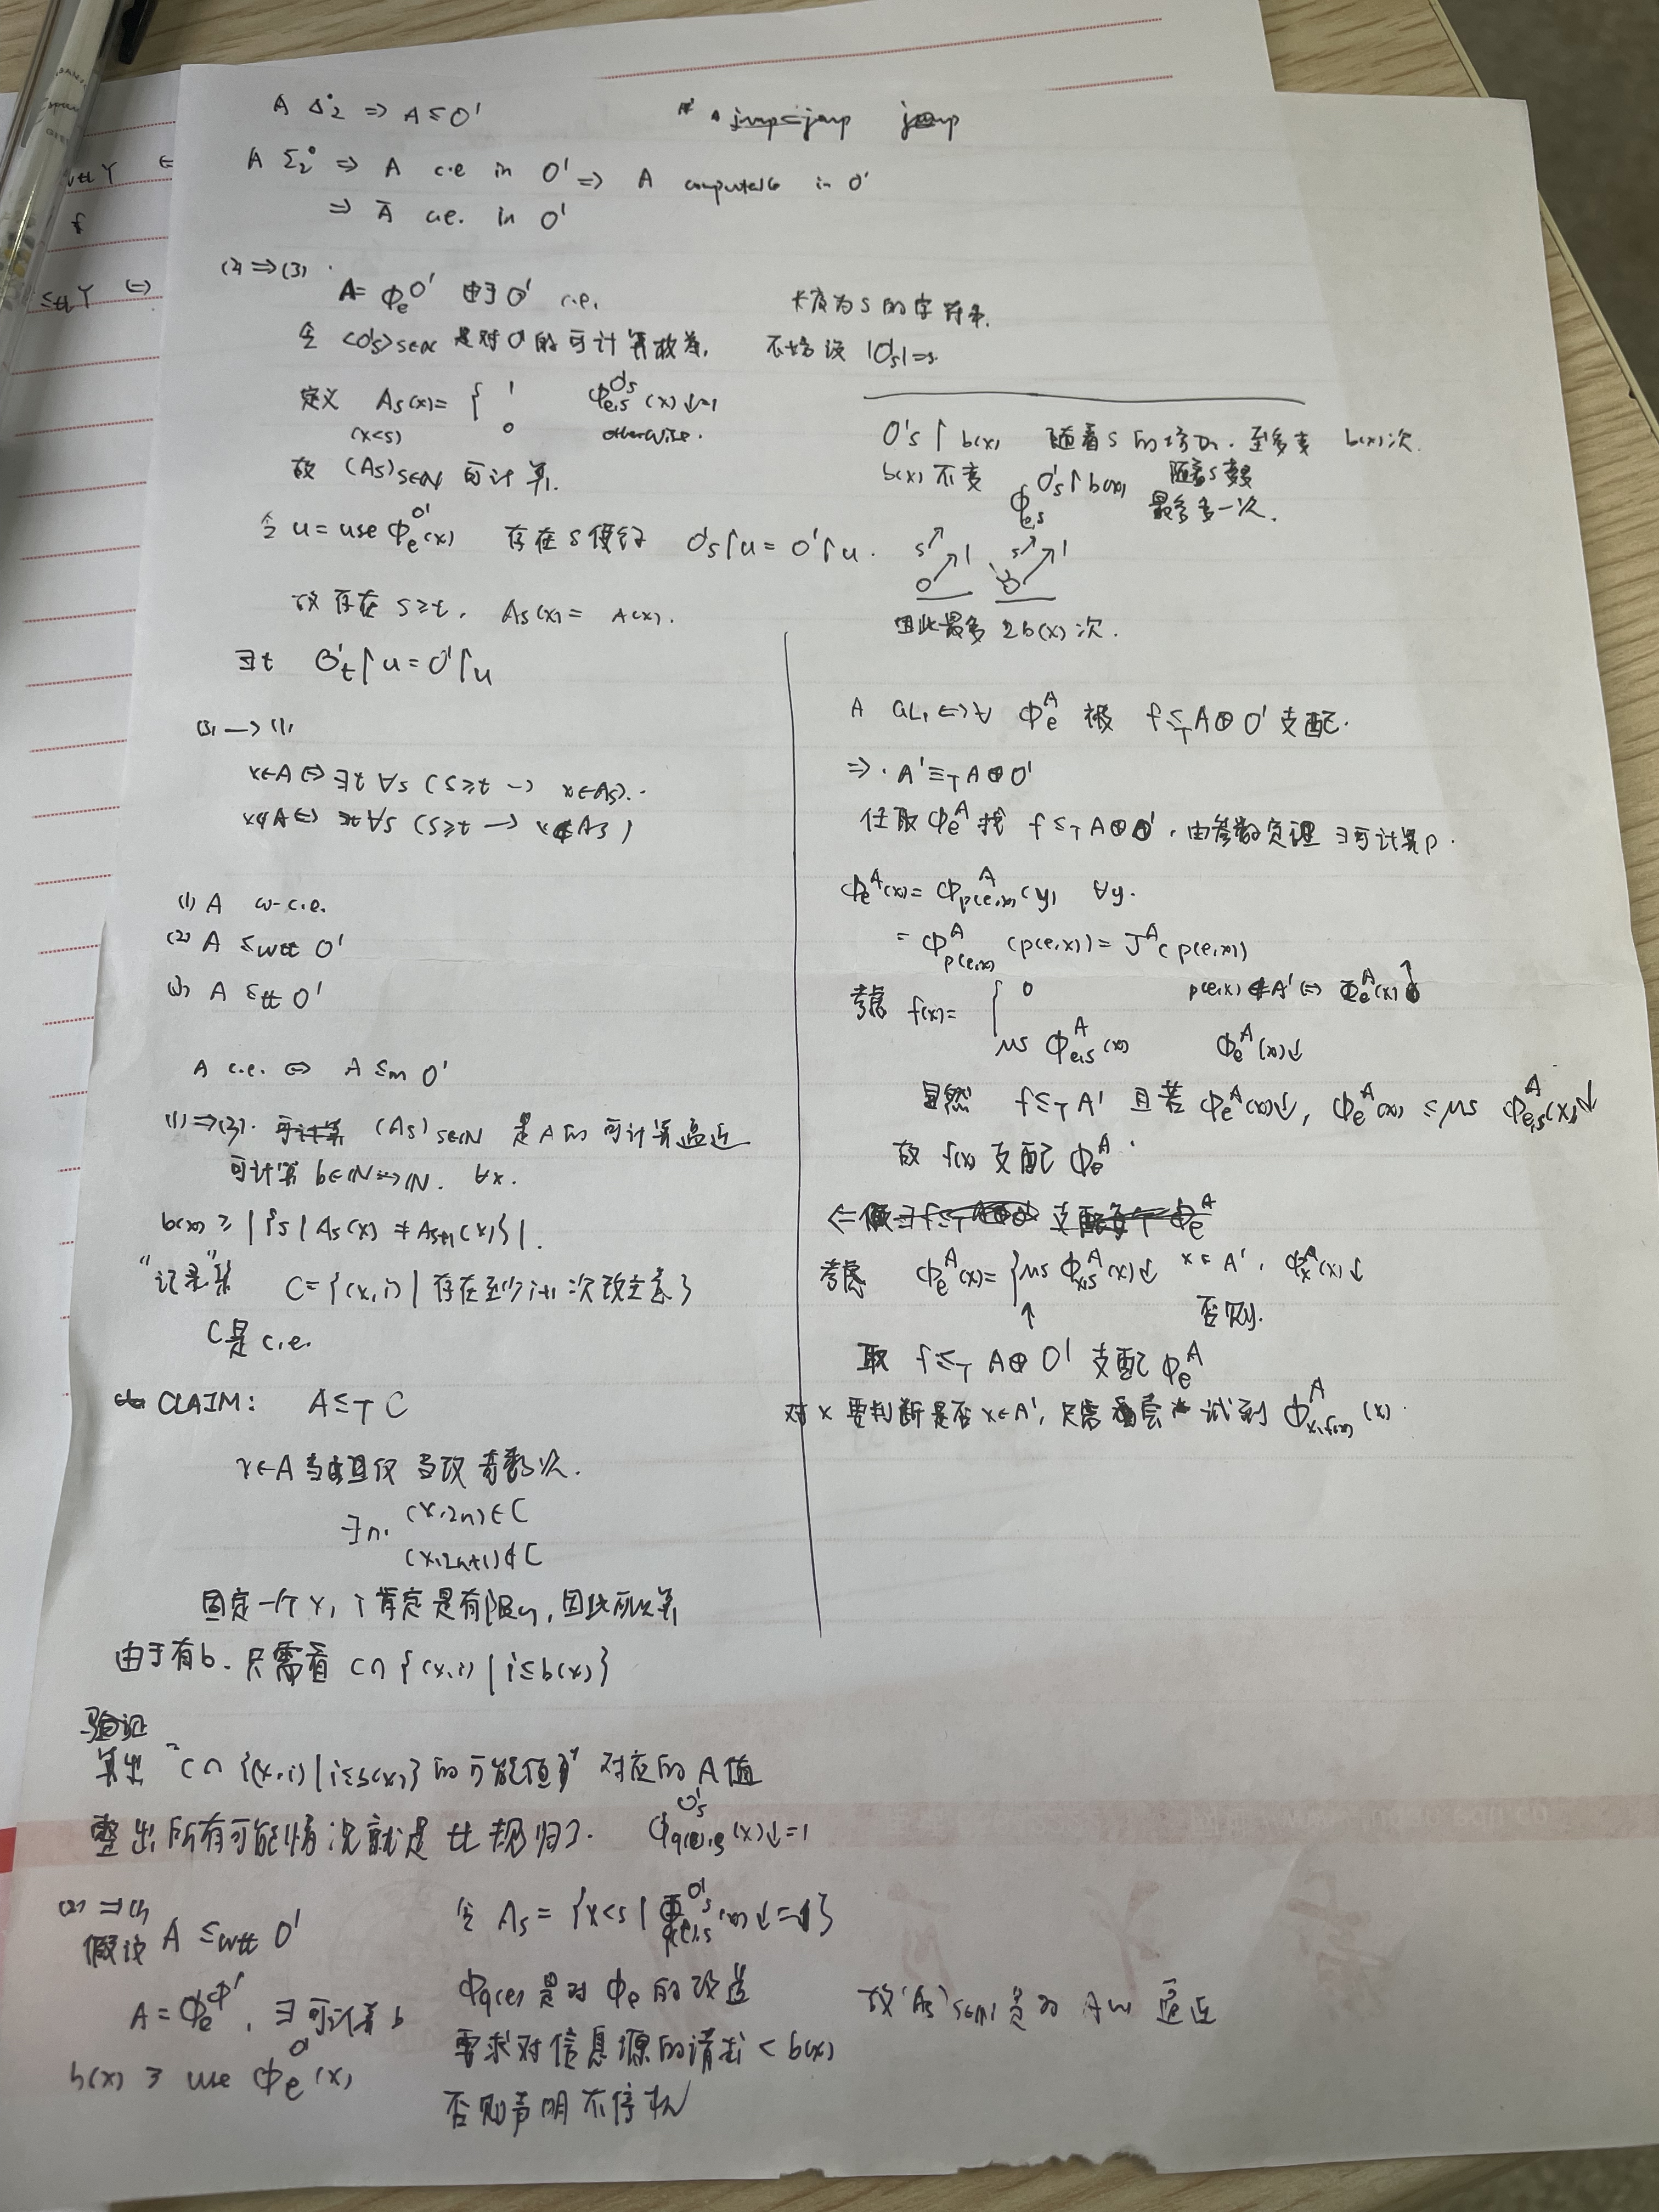
\includegraphics[width=.8\textwidth]{./1.png}
\label{}
\end{H}
\end{frame}

\begin{frame}[label={sec:orgfdcc0fb}]{参考资料}
\begin{itemize}
\item Knuth在stanford的\href{https://www.youtube.com/watch?v=mert0kmZvVM}{\color{blue}{授课视频}}。
\item Knuth, Donald Ervin, et al. \href{https://jmlr.csail.mit.edu/reviewing-papers/knuth\_mathematical\_writing.pdf}{\color{blue}{Mathematical writing}}。
\item Halmos, Paul R.  \href{https://entropiesschool.sciencesconf.org/data/How\_to\_Write\_Mathematics.pdf}{\color{blue}{How to write mathematics}}。
\end{itemize}
\end{frame}

\section{习题的一些问题}
\label{sec:org6cd751d}
\begin{frame}[label={sec:org306206c}]{名言警句}
    \begin{displayquote}
Often the experience of learning of the Model theory is similar to the one of learning of Physics: for a [short] while everything is so simple and so easily reformulated in familiar terms that “there is nothing to learn” but suddenly one find himself in a place when Model theoreticians “jump from a tussock to a hummock” while we mathematicians don't see where to “put a foot” and are at a complete loss.\par
\hfill David Kazhdan. Lecture notes in motivic integration
    \end{displayquote}
\end{frame}
\begin{frame}[label={sec:orga35d86b}]{一张图}
\begin{center}
\begin{H}
\centering
\includegraphics[height=.8\textheight]{./3.jpeg}
\label{}
\end{H}
\end{center}
\end{frame}
\begin{frame}[label={sec:org4ca446e}]{证明两个集合相等}
如果我们要证明两个集合\(A\)和\(B\)相等,我们现在的工具只有外延原理。

\vspace{5mm}
\alert{外延原理} :\(A=B\)当且仅当\(A\)和\(B\)有相同的元素。

\vspace{5mm}
证明:如果\(X\subset Y\),那么\(X\cap Y=Y\)。

\vspace{5mm}
思路:由外延原理可知,我们要证明\(X\cap Y=Y\),我们就要证明\(X\cap Y\)的所有元素属于\(Y\)并且\(Y\)的所
有元素属于\(X\cap Y\),即我们要证明\(X\cap Y\subset Y\)并且\(Y\subset X\cap Y\)。
\end{frame}
\begin{frame}[label={sec:orgbf189b5}]{交与一般交}
考虑\(\calf=\{X_i\mid i\in\N\}\),对\(i\in\N\),定义\(Y_i=\bigcap_{j\le i}X_j\)。证明:\(\bigcap\calf=\bigcap_{i\in\N}Y_i\)。

\vspace{5mm}
有同学试图这样表示一般交
\begin{equation*}
\bigcap\calf=X_1\cap X_2\cap\cdots\cap X_n\cap\cdots
\end{equation*}

\vspace{5mm}
我们来看这为什么是错的。
\end{frame}
\begin{frame}[label={sec:orgac449ec}]{交与一般交}
\begin{definition}[]
如果\(A\)和\(B\)是集合,那么\(A\)与\(B\)的 \alert{交集} 为
\begin{equation*}
A\cap B=\{x:x\in A\text{ 并且 }x\in B\}
\end{equation*}

对于集合族\(\calf=\{F_i:i\in\N\}\),它的 \alert{一般交} 为
\begin{equation*}
\bigcap\calf=\{x:\text{对于每一个}F\in\calf,\text{我们有}x\in F\}
\end{equation*}
\end{definition}
\end{frame}


\begin{frame}[label={sec:org880fb9f}]{交与一般交}
我们可以看到,交这个操作是作用在两个集合上的,但同时我们可以用它表示有限个元素的交。
对于有限个集合\(A_1,A_2,\dots,A_n\),
\begin{equation*}
A_1\cap A_2\cap\cdots\cap A_n=A_1\cap(A_2\cap(\cdots\cap(A_{n-1}\cap A_n)\cdots))
\end{equation*}
而对于集合族\(\calf=\{A_1,A_2,\dots,A_n\}\),我们可以证明
\begin{align*}
\bigcap\calf&=\{x:\text{对于每一个}A_i\in\calf(i\in\{1,2,\dots,n\}),\text{我们有}x\in F\}\\&=A_1\cap A_2\cap\cdots\cap A_n
\end{align*}
因此对于有限个元素,它们的交与仅包含它们的集合族的一般交是一样的。
\end{frame}
\begin{frame}[label={sec:org27521d1}]{交与一般交}
但是对于无穷个集合\(\{X_i\}_{i\in\N}\),因为交操作只能在作用有限个集合上,因此我们无法利用交操作得到所
有集合的交集。

\vspace{5mm}因此我们不能把\(\bigcap\calf\)表示为
\begin{equation*}
X_1\cap X_2\cap\cdots\cap X_n\cap\cdots
\end{equation*}
\end{frame}
\begin{frame}[label={sec:org6a36110}]{并与一般并}
并与一般并分别依赖于对集公理和并集公理。
\end{frame}
\begin{frame}[label={sec:org3699021}]{偏序与严格偏序}
\begin{definition}[]
令\(\le\)为\(X\)上的二元关系,如果\(\le\)满足
\begin{enumerate}
\item \(\le\) 是自反的,即对所有的\(x\in X\),\(x\le x\)。
\item \(\le\)是反对称(antisymmetric)的,即对所有的\(x,y\in X\),如果\(x\le y\)且\(y\le x\),则\(x=y\)。
\item \(\le\)是传递的,即对所有的\(x,y,z\in X\),如果\(x\le y\)且\(y\le z\),则\(x\le z\)。
\end{enumerate}


就称\(\le\)是\(X\)上的一个 \alert{偏序} 。
\end{definition}
\end{frame}
\begin{frame}[label={sec:org78a5afa}]{偏序与严格偏序}
\begin{definition}[]
令\(<\)为\(X\)上的二元关系,如果\(<\)满足
\begin{enumerate}
\item \(<\) 是非自反的,即对所有的\(x\in X\), \(x< x\)不成立。
\item \(<\)是非对称(asymmetric)的,即对所有的\(x\), \(y\in X\),如果\(x< y\),那么并非\(y<x\)。
\item \(<\)是传递的,即对所有的\(x\),\(y\),\(z\in X\),如果\(x< y\)且 \(y< z\),则\(x< z\)。
\end{enumerate}


就称\(<\)是\(X\)上的一个 \alert{严格偏序} 。
\end{definition}
\end{frame}
\begin{frame}[label={sec:org64f5ad2}]{偏序与严格偏序}
对于这两个定义,我们要关注反对称和非对称这两个性质。在非自反的条件下,这两个性质是等价的。

\begin{proposition}[]
令\(R\)是\(X\)上的二元关系,如果\(R\)是非自反的,那么\(R\)是反对称的当且仅当\(R\)是非对称的。
\end{proposition}
\end{frame}
\begin{frame}[label={sec:org01e9b27}]{偏序与严格偏序}
\begin{proposition}[]
令\(R\)是\(X\)上的二元关系,如果\(R\)是非自反的,那么\(R\)是反对称的当且仅当\(R\)是非对称的。
\end{proposition}

\begin{proof}
\begin{enumerate}
\item 如果\(R\)是反对称的,我们使用反证法,如果存在\(x\),\(y\in X\)使得\(xRy\)且\(yRx\),于是\(x=y\),于是我
们有\(xRx\),与自反性矛盾。
\item 如果\(R\)是非对称的,对于任意\(x,y\in X\),如果\(xRy\)并且\(yRx\),我们知道这是错误的,于
是\(R\)是反对称的。
\end{enumerate}


因此在非自反的条件下,这两个概念是等价的。
\end{proof}
\end{frame}

\begin{frame}[label={sec:orgade6248}]{推荐阅读}
\href{https://web.stanford.edu/class/archive/cs/cs103/cs103.1198/handouts/070\%20Guide\%20to\%20Set\%20Theory\%20Proofs.pdf}{\color{blue}{Guide to proofs on sets}}
\end{frame}
\end{document}
